\Chapter{Implementáció}

A Harmadik fejezet alapján a felhasználó naprakész háttérinformációval rendelkezik a fejlesztési folyamattal és a szükséges technológiák ismeretével kapcsolatban. Ezen ismeretek megszerzésével ebben a fejezetben prezentálni fogom az elkészült alkalmazás látható és háttérmunkaként szolgáló programrészeit.


\section{Áttekintés}

A szakdolgozatom témája interaktív megjelenítő eszköz (ez esetben weboldal) pénzügyi adatok elemzéséhez. Ilyen szoftverekből különféle megvalósítást lehet találni az Interneten, amelyeket nagyobb befektetői háttérrel rendelkező cégek működtetnek általában valamilyen pénzbeli szolgáltatás ellenében. Számomra elsődleges szempontot képviselt a szabad és pénzmentes felhasználás, a könnyű kezelhetőség, átláthatóság és sokszínűség, különösképpen a grafikont illetően. A már bemutatott Chart.js technológia nagyszabású könyvtárának ismeretével megalkotott gráfok több lehetőséget is a felhasználó elé tárnak, mind megjelenés, mind adathalmazok terén. 

\subsection{Problémakör}

Ahogy az Áttekintésben felvázoltam több grafikonrajzoló és eszközkezelő weboldal létezik napjainkban. Ezen oldalakat vizsgálva feltűnt, hogy több megkötés árán tudtam hozzájutni a kívánt adatokhoz. Az egyik ilyen megkötéssel akkor szembesültem, amikor a grafikonrajzolóhoz nem engedett hozzáférni felhasználó nélkül. Mivel teljes mértékben piackutatás céljából vizsgálódtam, nem tartottam fontos szempontnak felhasználó regisztrálását, így az oldal használatát a továbbiakban nem tudtam folytatni.

	Következő korlátozás amivel találkoztam, mely szerint a biztosítási cégek által használt webhelyek részvények és portfóliók széles körű tárházával rendelkeznek, de jogi és piaci okokból kifolyólag korlátozott az adatbázisuk, hiszen más vállalatok termékeit nem híresztelhetik. Kutatásaim során meggyőződtem, hogy ezen adatok nyilvánosak az ügyfelek számára, tehát illusztrálásuk engedélyezett bármely kliens részére.

	Továbbiakban széleskörű adatforrással rendelkező portálokat után keresgéltem és sikeresen találtam pár ilyen paraméterekkel rendelkező weboldalakat. Azonban túlnyomórészt idegen nyelven íródtak, ami globális szinten érthető megközelítés, viszont mint magyar anyanyelvű felhasználó ezt problémának éreztem. 

\subsection{Program működésének elve}

Ebben az alfejezetben pár szóval ismertetem, hogy az alkalmazást milyen felhasználói körnek hoztam létre első sorban. Alapvetően adatbányász, tőzsdei jelenléttel rendelkező vállalatoknak ajánlanám, hiszen korlátozás nélkül bővíthető az adathalmaz, ezáltal optimalizálható bármely piaci részre. Struktúrájában kulcsszerepet képviseltek az alábbi szempontok.

\begin{itemize}
\item \textbf{Megjelenés}: Felépítése, megjelenése letisztult és modern, jelképezve egy innovatív oldal benyomását.
\item \textbf{Reszponzivitás}: Weboldalam célja, hogy optimális megjelenést biztosítson \\
(könnyű olvashatóság, egyszerű navigáció) a legkülönfélébb eszközökön át az asztali számítógépektől egészen a mobiltelefonokig. Az oldal tökéletesen igazodik a megjelenítő eszközhöz a rugalmas felépítésével és flexibilis képeivel.
\item \textbf{Egységes színvilág}: A színvilág megvalósításánál elengedhetetlen tényező volt, hogy a felhasználónak kellemes színeket használjak, amelyek harmonizálnak egymással. Szubjektív kikötésem volt a fehér háttérszín elvetése, mert számomra szemvakító.
\item \textbf{Egységes formavilág}: Az egész weboldalnak egységes a formavilága, könnyen felismerhető panelekkel felépítve. A gombok, képek és szöveg megjelenése nem tér el panelenként szemben sok más alkalmazással.
\item \textbf{Navigálhatóság}: A weblap összes panele könnyen elérhető akár a navigációs sáv használatával, akár az oldalak közti kommunikációval.
\item \textbf{Funkciók}: Implementált funkciók szerepüket működésük szerint betöltik, bármely böngészőn futtatjuk az alkalmazást.
\item \textbf{Tartalom}: Releváns és minőségi értéket ad a látogató számára.
\item \textbf{Honlapszerkezet}: Az oldalak hierarchikusan vannak felépítve, tehát logikusan következnek egymásból.
\end{itemize}

\section{Fejlesztési eszközök}

Webfejlesztőként arra törekedtem, hogy modern weboldalt hozzak létre. Ezt a szempontot nem csak kódolás, hanem a kijelölt feladatok megvalósításánál is szem előtt tartottam, mint például a kliens és a szerver kezelése. Az alkalmazás során több webfejlesztő eszköz segítette a fejlesztés teljes folyamatát. A következő modulban ezeket az eszközöket fogom bemutatni.

\subsection{Részvények adataihoz való hozzáférés}

A részvények adatainak az igénybe vételét külsős oldal segítségével oldottam meg. Az oldal amit használok az \emph{EOD Historical Data}, amely egyszerű hozzáférést biztosít az alapvető tőzsdei adatokhoz és az országokból származó részvényekhez és befektetési alapokhoz. Az oldalon található adatok védettek, ezért egy biztonsági eljárás útján tudom elérni őket. Ezen eljárás alapján a regisztrált felhasználómhoz az oldal generál úgy nevezett "API KEY"-t, ami minden felhasználónak egyedi és elengedhetetlen része az adatokat lekérő URL-nek. Miután megszereztem az kulcsot a lekérdezésben feltétlenül szerepelnie kell, különben nincs jogosultságunk az adatok eléréséhez.  \cite{eod} \\

\begin{figure}[h]
\centering
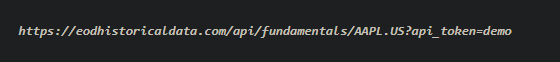
\includegraphics[scale=0.9]{images/demoAPI.png}
\caption{API hívás demo ID-val (forrás:\cite{eod})}
\end{figure}

	Elérhető fizetős és ingyenes változata is, én az utóbbit használom, aminél némi megkötéssel kellett szembesülnöm, mint például a maximum időintervallum, amire az API-hívások szólhatnak az 1 év, tehát a grafikon ábrázolásának van határa. Ezen felül naponta csak 20 hívást tudok intézni, így erre a problémára egy megoldással kellett előállnom, amit a \textbf{Szerver} szekcióban fogok ismertetni.

\subsection{Postman}

A fenti részben említett API hívásokat külső applikációval valósítom meg, ez pedig a \emph{Postman}. A Postman az egyik legnépszerűbb szoftvertesztelő eszköz, amelyet API tesztelésére, létrehozására, megosztására és dokumentálásra alkalmaznak a fejlesztők. 

	Működését tekintve igen egyszerű a használata. Elsőként ki kell választani milyen típusú hívást akarunk intézni, mivel adatokat szeretnék elérni, ezért "GET" kéréssel hivatkozok. Továbbiakban szükségem van az elérni kívánt weboldal URL címére. Következő feltételhez tőzsdei ismeretek szükségesek. Minden nyilvánosan működő részvénytársaság regisztrálva van a globális piacon, ezáltal regisztrációs címmel, úgy nevezett "TOKEN"-nel rendelkeznek, például a legismertebb tőzsdei token a TSLA, nevéből kifolyólag a TESLA részvényeire vonatkozik (\aref{fig:postman}). Ezen teendők után meg kell adni a kéréshez tartozó időtartam kezdeti és záró dátumát, ha nem adjuk meg a záró dátumot, akkor a lekérés automatikusan az aktuális napot állítja be. 

\begin{figure}[h]
\centering
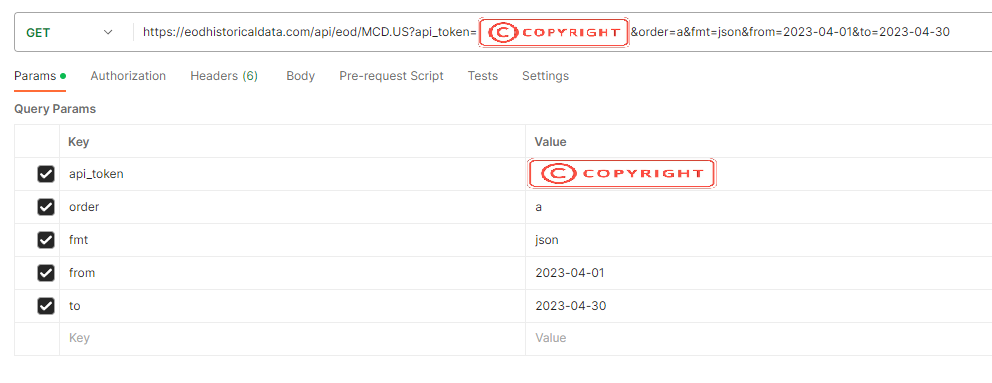
\includegraphics[scale=0.5]{images/postman.png}
\caption{Adatok lekérése Postman használatával (adatvédelmi okokból cenzúráztam a kulcsot)}
\label{fig:postman}
\end{figure}

\pagebreak

\subsection{Fejlesztői környezet }

A \textbf{Visual Studio Code} nyílt forráskódú kódszerkesztő, mely ingyenesen elérhető a fejlesztők számára. Az egyik legnépszerűbb alkalmazás, hiszen számos kiegészítővel rendelkezik, amely leveszi a terhet a felhasználó válláról, továbbá majdnem az összes ismert programozási nyelvet támogatja, például az általam is használt JavaScriptet, HTML-t, CSS-t és Node.js-t. 

A VS Code beépített támogatást tartalmaz az intelligens kódkezelésre az IntelliSense segítségével, mely nem csak a kód kiegészítésében és refaktorálásában, de a navigációban is hasznos lehet, főleg egy összetettebb projekt kapcsán. Ezenkívül beépített támogatást tartalmaz Node.js hibakereséshez és JavaScript fejlesztéséhez. Ezeken felül lehetőségünkben áll bővítményeket hozzáadni, mint például \emph{Live Server}, illetve rendelkezik beépített parancssorral, melyből így futtathattam a Node.js kódomat. \cite{vsc}

\subsubsection{Live Server}

A Visual Studio Code Elő Szerver (Live Server) bővítménye hihetetlenül hasznos a webfejlesztés folyamat során. Lehetővé teszi, hogy egy kattintással elindítsunk egy HTML dokumentumot és lefuttat egy dinamikusan generált szervert, amely során megnyit egy böngésző ablakot és feltölti az általunk kódolt elemekkel. A fájlon végrehajtott bármilyen gyakorlati módosítást követően a böngésző ablakát újratölti és azonnal végrehajtja a változtatásokat. 

\subsection{Git }

A Git ingyenes, nyílt forráskódú verziókezelő rendszer, amelyet a kis és közepes projektek hatékony kezelésére használnak. A Git a forráskód változásainak nyomon követésére szolgál, lehetővé téve több fejlesztő számára, hogy együtt dolgozzon a fejlesztésen. Lényeges funkciója a verziókezelésen felül a Git folyamat elágazási stratégia (flow branching strategy), amely hierarchikus kapcsolatot hoz létre a különböző könyvtárak és fájlok között. Ezáltal a fejlesztési folyamatokat külön ágakon lehet végezni, így elkerülhető az esedleges hibás kódolás terjesztése többi fejlesztő számára. Néhány fontosabb információ a Git-tel kapcsolatban: 

\begin{itemize}
\item Az elosztott verzióvezérlő eszköz a forráskód-kezelésre szolgál
\item Lehetővé teszi több fejlesztő együttműködését
\item Több ezer párhuzamos ágán keresztül támogatja a nemlineáris fejlesztést
\item Nyomon követi az előzményeket, illetve biztonsági mentéseket készít \cite{git}
\end{itemize}

Az általam készített alkalmazást regisztráltam a GitHub felhő alapú szolgáltatásán, amely tárolja a szükséges kódokat és fájlokat. Fejlesztésem során több ágon (branch) dolgoztam, így a forráskód csakis abban az esetben került fel a fő (main) ágamra, ha a mellékágakon tesztelési folyamatok után sem találtam hibát.

\section{Kliens}

Először a Kezdőlap és Grafikonrajzoló oldalak funkcióival kezdtem a tervezést. Az \emph{index.html} fájlban létrehoztam a navigációhoz tartozó paneleket, majd CSS felhasználásával megalkottam a kinézetét és azt a kritikus funkciót, hogy a navigáció mindig a képernyő tetején legyen, és kövesse annak a mozgását, így a felhasználó könnyedén tud lapozni az oldalak között. Mivel az oldalamat több felbontásra terveztem a reszponzivitás szemléletében, következésképpen itt is kulcs szerepet tölt be. Mivel a betűk eléggé nagyok, ezáltal bizonyos felbontás mellett egymásra halmozódnának, ezt elkerülve, ha az képernyő mérete kisebb mint, 1099 px, akkor a navigáció összecsukódik egy kis gombbá és a soros megjelenítést felváltja az oszlopos megvalósítás (\aref{fig:navbarfunc}).

\begin{figure}[h]
\centering
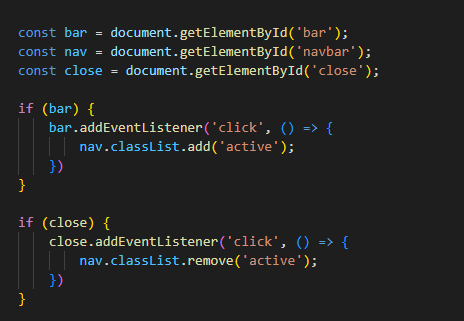
\includegraphics[scale=0.8]{images/navbarFunction.png}
\caption{A navigációs sáv összecsukása és kinyítása}
\label{fig:navbarfunc}
\end{figure}

További fejlesztés volt még az oldalak HTML vázának megvalósítása. Szükséges szempont volt, hogy a különböző oldalak más elemekkel töltsem fel, de alapjában véve egységes weboldal látszatát keltsék. A különböző részeket <section> címkével (tag) választom el, így átláthatóbb számomra, illetve néhány szekciót egyedi azonosítóval (id) láttam el, hogy működésüket, vagy külsejüket tudjam applikálni. A gombok és választható elemeknél a \textbf{Bootstrap} könyvtár beépített függvényeit használtam. A dátumokhoz tartozó gombokat jQuery függvény segítségével kiszelektálom és megjelenítek hozzájuk egy naptárat is. A naptáron lehetőség van kattintással kiválasztani a napot, vagy váltani a hónapok és évek között, illetve ha mégsem a megfelelő dátum lett kiválasztva, akkor a törlés gomb megnyomásával hatálytalanítjuk a bevitt adatot (\aref{fig:datepicker}).

\begin{figure}[h]
\centering
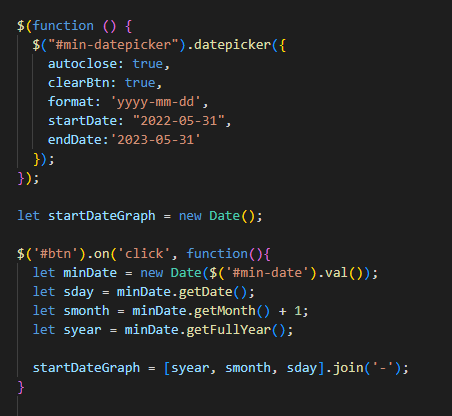
\includegraphics[scale=0.7]{images/datepicker.png}
\caption{A dátumválasztó működése kezdő dátumra}
\label{fig:datepicker}
\end{figure}

\pagebreak

A kliens egy API-n keresztül (\aref{fig:apiCall}), HTTP kérésekkel kommunikál a szerverrel. A kommunikáció úgy néz ki, hogy a \textbf{Grafikonrajzoló} oldalon található gomb megnyomásával inicializáljuk a rajzolót egy aszinkron függvény használatával. A függvény csak akkor hívódik meg, ha a felhasználó beállította a programhoz elengedhetetlen adattagokat, ilyen adattagok például a grafikon típusa, valamelyik befektetési alap és az árfolyamok közül az egyik kiválasztása, illetve a kezdeti és záró dátumok. Hogy ne kelljen minden egyes alkalommal minden adattagot újra beállítani, így alapértelmezetten kiválasztottam az első három opcióbol egyet.
	
	Az aszinkron függvény megvizsgálja, hogy a gomb felett található kettő dátum input fel van töltve adatokkal, tehát a felhasználó kiválasztotta a kezdő és a záró dátumot (\aref{fig:validation}).

\begin{figure}[h]
\centering
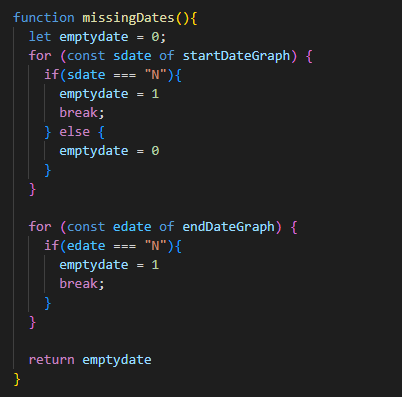
\includegraphics[scale=0.75]{images/dateValidation.png}
\caption{A missingDates függvény. megvizsgálja, hogy nincs-e üres dátum mező}
\label{fig:validation}
\end{figure}

Abban az esetben, ha üresek, akkor egy figyelmeztető üzenet jelenik meg, ami felhívja a figyelmet a dátumok kitöltésének követelményére. További feltételek még, hogy a kezdeti és záró dátum nem eshet ugyan arra a napra, illetve a záró dátum nem lehet kisebb, mint a kezdeti dátum, hiszen az API hívásban problémát okozna a hibásan megadott időintervallum.

\begin{figure}[h]
\centering
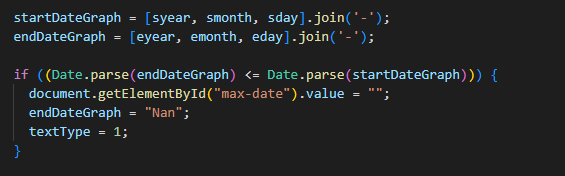
\includegraphics[scale=0.9]{images/emptyDate.png}
\caption{A kód felülvizsgálja a záró dátumot}
\end{figure}

Amennyiben minden mező sikeresen ki lett töltve, a program "GET" kéréssel lekéri az adatokat a szerverről és átadja a weboldal címét, a felhasználó által kiválaszott tokent és a kezdeti, illetve a végső dátumokat. 

\begin{cpp}
const url = `http:/localhost:8080/api?ticker=${selectedInvest}&
             &start_date=${startDateGraph}&end_date=${endDateGraph}`;
\end{cpp} 

Ha sikerült a kérés és nem merült fel semmilyen hiba, akkor a függvény Promise-szal (ígéret) jelzi, hogy minden adat elérte a weboldalt (\aref{fig:fetch}). Ezen adatokat a program JSON formátumban küldi el, csakúgy, mint ahogy backenden tárolva vannak, azzal a különbséggel, hogy csak azok az adattagok jöttek fel, amit a felhasználó kíválasztott.

\begin{figure}[h]
\centering
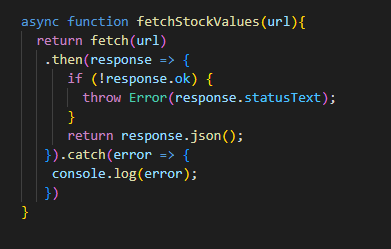
\includegraphics[scale=0.8]{images/fetch.png}
\caption{Backendről felküldött adatokat adja át a frontendnek JSON formátumban}
\label{fig:fetch}
\end{figure}

Most, hogy minden kért adat sikeresen elérte a klienst, következhet a diagram struktúrájának összetétele. Elsőként egy függvény felel azért, hogy meg tudjuk milyen típusú adatok lettek kiválasztva. Ez a függvény mindig meghívódik gombnyomás előtt, hogy inicializálja a gárfot, ha esetleg az alapértelmezett opciók helyett más lehetőséget választott volna a felhasználó, majd utána gombnyomásra aktiválódik a folyamat újra.

\begin{figure}[h]
\centering
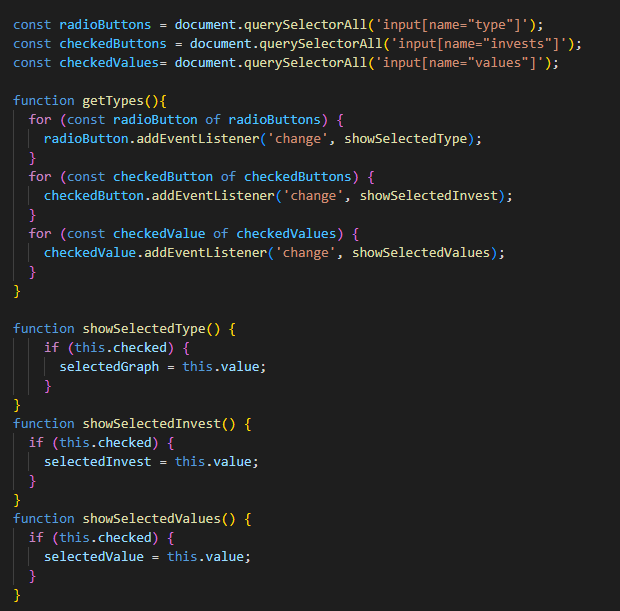
\includegraphics[scale=0.6]{images/types.png}
\caption{A getTypes függvény a diagram típusainak változását figyeli}
\label{fig:fetch}
\end{figure}

\pagebreak

A grafikon megvalósításához a Chart.js definiált könyvtárát használom fel. Ehhez HTML oldalon szükséges <canvas> címkét létrehozni, hiszen két dimenziós ábrát szeretnék megvalósítani. Egyedi azonosítóval láttam el a canvas elemet, amire a \emph{script.js} fájlban hivatkozok. A grafikonnak három fontos paraméterrel rendelkezik, úgy mint a típusa (types), adathalmaza (data) és opciói (options).

	A típusát "switch" választási mechanizmussal érem el aképpen, hogy a felhasználó melyik befektetést választotta ki az oldalon, úgy az ahhoz tartozó megnevezést adom át a grafikonnak. 
Az adathalmazt egy függvény segítségével töltöm fel. Az API hívás során megkapott JSON fájlon végigiterál a függvény és egy tömbben adja vissza az adatokat amivel a grafikon tud dolgozni (\aref{fig:chartData}). Az opcióit JSON formátumban használom. A grafikon felett megjelenített idősávot függvény során valósítom meg, ami mindig a felhasználó által kiválasztott aktuális dátumot jeleníti meg, feltéve ha a dátumok megfelelnek a hibaellenőrzésnek. Animációval teszem látványosabbá a diagrammok megjelenítését.

\begin{figure}[h]
\centering
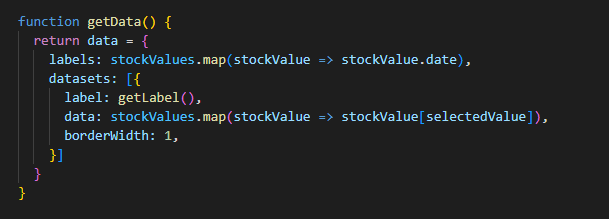
\includegraphics[scale=0.8]{images/chartData.png}
\caption{Az API hívás során megkapott adathalmazon iterál végig a getData függvény}
\label{fig:chartData}
\end{figure}

Az alkalmazás struktúrája úgy működik, hogy minden alkalommal amikor a "Mehet" gombot megnyomja a felhasználó az addig használt gráf úgymond megsemmisül, és helyette a program új gráfot készít a megadott paraméterekkel (\aref{fig:newChart}). Természetesen a feltételvizsgálat itt is fontos szerepet játszik, tehát ha nincs megadva dátum, akkor hiba üzenet fog megjeleni és a gráf törlődik.

\begin{figure}[h]
\centering
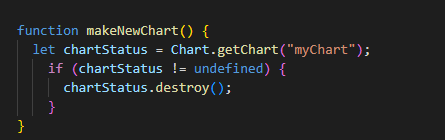
\includegraphics[scale=0.8]{images/makeNew.png}
\caption{A függvény megvizsgálja, hogy létezik gráf, ha igen, akkor törli azt}
\label{fig:newChart}
\end{figure}

\section{Szerver \label{fig:server}}

Ahhoz, hogy a szoftver működjön telepítenünk kell a megfelelő technológiákat. Ahogy már a \textbf{Bevezetőben} ismertettem, a kliens-szerver architektúra megfelelő az alkalmazásra. A kliens egy böngészőben futtatott frontend, ami API hívásokon keresztül tud kommunikálni a backend szerverrel.
Hogy az architektúra működjön a számítógépünkön először telepíteni kell a Node.JS-t, és az Express-t. A Node.js-t egyszerűen le lehet tölteni a hivatalos honlapról \cite{nodeJS}. Windows-os felhasználóként az ehhez az operációs rendszerhez készített 64-bites setup segítségével telepítettem fel az alkalmazást. Hogy megbizonyosodjunk a \emph{Node.js} sikeres letöltésről (\aref{fig:node}) bemutatok egy próba tesztet.

\begin{figure}[h]
\centering
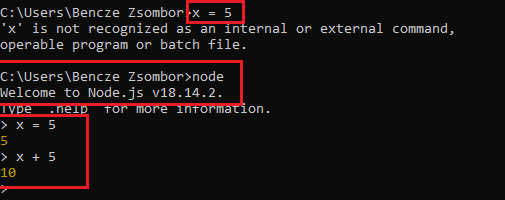
\includegraphics[scale=0.9]{images/nodeTest.png}
\caption{Sikeresen telepített node demó}
\label{fig:node}
\end{figure}

Miután megbizonyosodtunk, hogy sikeresen telepítettük a Node.js aktuális verzióját, használjuk a Visual Studio Code, vagy a Windows beépített terminálját és írjuk be a következő parancsot:
\begin{cpp}
npm init
\end{cpp} 
A kód lefutása után lehetőségünkben áll csomag nevet (package name), verziót (version), leírást (description), belépési pontot (entry point), teszt parancsot (test command), git adattárat (git repository), kulcsszavakat (keywords), szerzőt (author) és licenszt (license) megadni, de én azt javaslom az enter megnyomásával mindent hagyjunk meg a rendszernek, hogy automatikusan töltse ki helyettünk. Ha mindent jól csináltunk akkor létre kellett jönnie egy \emph{package.json} fájlnak (\aref{fig:package}). A telepítésünk következő lépése a az \emph{Express.js} installálása, amit szintén a terminálon keresztül tudunk letölteni az alábbi paranccsal:
\begin{cpp}
npm install express --save
\end{cpp}

\begin{figure}[h]
\centering
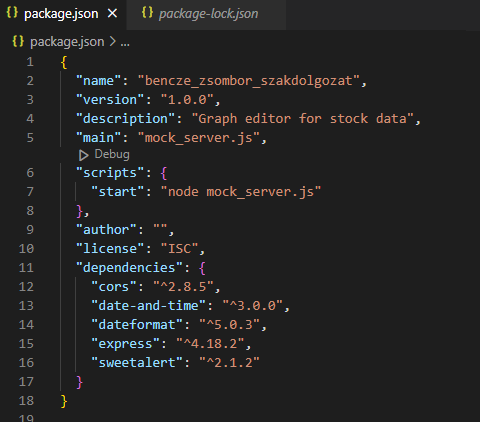
\includegraphics[scale=0.9]{images/packageJSON.png}
\caption{Az alkalmazáshoz készített package.json }
\label{fig:package}
\end{figure}

Észrevehetjük, hogy egy új mappa \emph{node\_modules} ékelődött be a fájlaink közé. Ez egy könyvtár, amelyet az npm hozott létre, és egy módja annak, hogy nyomon kövesse a helyileg telepített csomagokat. A felhasznált csomagok nevei és verziószámai, mind a \emph{package.json} nevű fájlban találhatók így, ha a GitHubra akarom menteni a projekteket, akkor időt sprólok, hiszen nem nekem kell egyesével több ezer fájlt feltöltenem a felhőbe, mert mindegyik megtalálható lesz a JSON-ben. Az ábrán (\aref{fig:package}) látható dependenciák (dependencies) tartalmazza mindazokat a telepítéseket amiket az alkalmazáshoz használtam.

	A telepítést követően létre kell hoznunk a webszervert portját, amit az Express csomag segítségével létrehoztam. A szerver alapját úgy állítottam be, hogy a 8080-as porton figyeljen, azaz a böngészőben a http://localhost:8080 címen legyen elérhető (\aref{fig:serverPort}).

\begin{figure}[h]
\centering
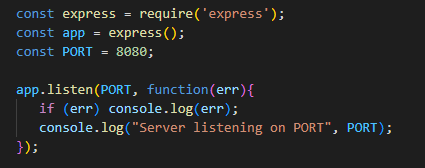
\includegraphics[scale=0.9]{images/serverPort.png}
\caption{Ezen a porton lehet elérni a szervert}
\label{fig:serverPort}
\end{figure}

\pagebreak

A szerver működtetéséhez már csak egy lépés van hátra, mégpedig létrehozni magát a tényleges HTTP szervert (\aref{fig:createServer}). A kódot úgy írtam meg, hogyha a szerver 200-as státuszkódot kap, tehát nem történt hiba a szerver elérésében, akkor a "req" argumentumot felhasználva a kód lekéri a klienstől az URL-t, továbbá meghív egy "getData" nevű függvényt, amit később fogok ismertetni. \cite{nodeServer}

\begin{figure}[h]
\centering
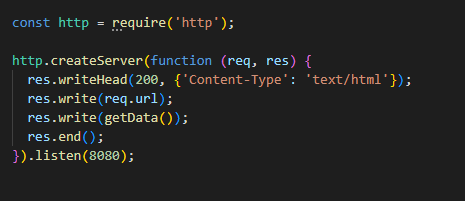
\includegraphics[scale=1]{images/createServer.png}
\caption{Szerver létrehozása}
\label{fig:createServer}
\end{figure}

A szerver REST API-n keresztül hallgat a kérésekre (\aref{fig:apiCall}). Ezen az API-n szolgálja fel a statikus tőzsdei adatokat, amiket backend/data mappába mentettem el és Postman  (\aref{fig:postman}) segítségével "GET" kéréssel értem el az adatokat. Mivel az alkalmazás hat különböző befektetést ismertet, így hat API hívást intéztem, amelyeket JSON fájlban tároltam, hogy könnyen feltudjam küldeni őket a kliensre.

\begin{figure}[h]
\centering
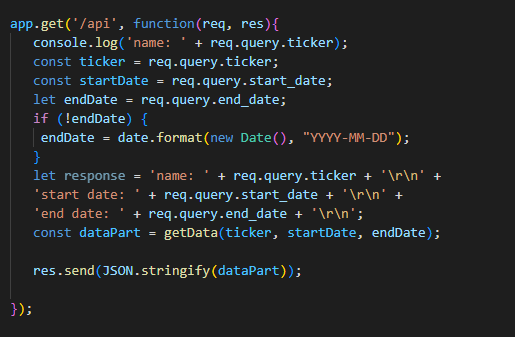
\includegraphics[scale=0.8]{images/apiCall.png}
\caption{Szerverről intézett API hívás}
\label{fig:apiCall}
\end{figure}

Mivel a szerver és a kliens nem egy URL címen futnak, ezért globálisan össze kell őket hangolni, amihez szükség van egy keresztező erőforrás megosztásra (Cross-Origin Resource Sharing) röviden: CORS. 

\begin{cpp}
let cors = require('cors')

app.use(cors({
   origin: '*'
}));
\end{cpp} 

\pagebreak

Most, hogy a szerver és a kliens is sikeresen kommunikál egymással, már csak egy lépés van hátra, mégpedig a felhasználó által igényelt adatok elérése. A weboldalon felhasználónak lehetősége adódik kiválasztani, hogy melyik befektetést szeretné megjeleníteni, illetve kitud választani két dátumot, miszerint mettől (kezdeti dátum input) meddig (záró dátum input) szeretné megjeleníteni a grafikonrajzolóval a kívánt gráfot. Majd ezeket a dátumokat a kliens leküldi a szervernek, amely megkapva feldolgozza és a kért paraméterek alapján megszűri az adott JSON-t, és úgy küldi vissza a kliensnek (\aref{fig:getData}).

\begin{figure}[h]
\centering
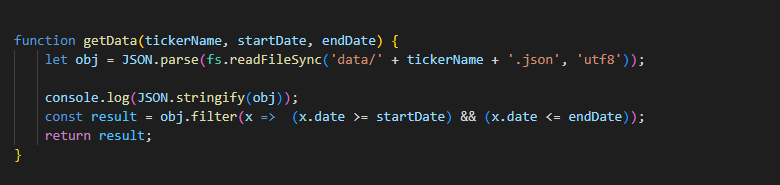
\includegraphics[scale=0.7]{images/getData.png}
\caption{Frontend-ről megkapott adatok alapján kiválasztja a kezdeti és záró dátumon belüli értékeket}
\label{fig:getData}
\end{figure}